\documentclass[10pt]{article}
\usepackage[margin=0.72in]{geometry}
\usepackage[T1]{fontenc}
\usepackage{lmodern,graphicx,amsmath,hyperref}
\hypersetup{colorlinks=true,urlcolor=blue}
\setlength{\parindent}{0pt}
\setlength{\parskip}{5pt}
\title{APS independent public-fixture replay}
\author{Native implementation follow-up}
\date{29 October 2026}
\begin{document}
\maketitle
\textbf{Question and boundary.} The earlier APS instrument checked results
with its own fast curve arithmetic. This continuation adds a separate native
replay path for its three existing public, known-answer fixtures. It checks
the mathematical transcript and sampling, while explicitly declining to
attest execution history or solver cost counters. No performance experiment,
scaling claim or new curve family is introduced.

\textbf{Method.} Strict parsing rejects unknown fields, duplicate or aliased
coordinate-map keys, unsupported metadata and oversized inputs. The checker
binds the fixture model, generator, target, public answer and ICV1 identity.
It uses existing BigUint field and point addition/doubling, with affine
double-and-add for known scalars; it never calls the producer's FastCurve,
sampler, polynomial solver or recovery routines.

For each attempt it regenerates the seeded label draws, discarded infinities
and repeated abscissae, partitions, sign representatives and orbit expansion.
The sign representative compares the Montgomery encoding of $y$ to $(p-1)/2$;
the verifier reproduces that convention with BigUint rather than assuming
the affine integer $y$ is the smaller lift. Every recorded point must satisfy
its independent label equation $R_i=u_iG+v_iQ$.

For every reported coordinate tuple the verifier enumerates signs and tests
the actual point sum. A tuple must satisfy the arm's partition or block
membership. A pruned line arm additionally excludes horizontal triples.
For a complete attempt it independently enumerates all allowed distinct
tuples and requires equality with the reported solution set. For a partial
attempt it validates the emitted subset and preserves partial status.

A recovery must bind to a reported tuple and its canonical sign orientation.
The checker recomputes $A=\sum s_i u_i$ and $B=\sum s_i v_i$, requires
$\sum s_iR_i=O$ and $B\ne0$, computes $d=-A/B\pmod n$, and checks $dG=Q$.
The public expected answer alone cannot authorize a relation: a horizontal
$B=0$ orbit remains a rejection even when its supplied $d$ is correct.

\textbf{Why the finite oracle covers the sign choices.} Every allowed tuple
has three or four distinct abscissae. Choosing one fixed lift per abscissa
leaves only its sign to select. Simultaneously negating all signs preserves
the zero-sum condition, zero/nonzero status of $B$, and recovered quotient.
Thus fixing the first sign positive covers every coordinate decomposition.
This applies the established group law; it is not a new mathematical result.

\textbf{Validation.} Final command receipts, failure history and source
digests are maintained in the study README and validation directory. The
tests cover independent sampling, fixture binding, complete and partial
sets, status/retry consistency, corrupted labels and witnesses, duplicate
JSON keys, resource bounds and every CLI arm in both enumeration modes.
Only completed checks in those receipts count as passed.

\newpage
\begin{center}
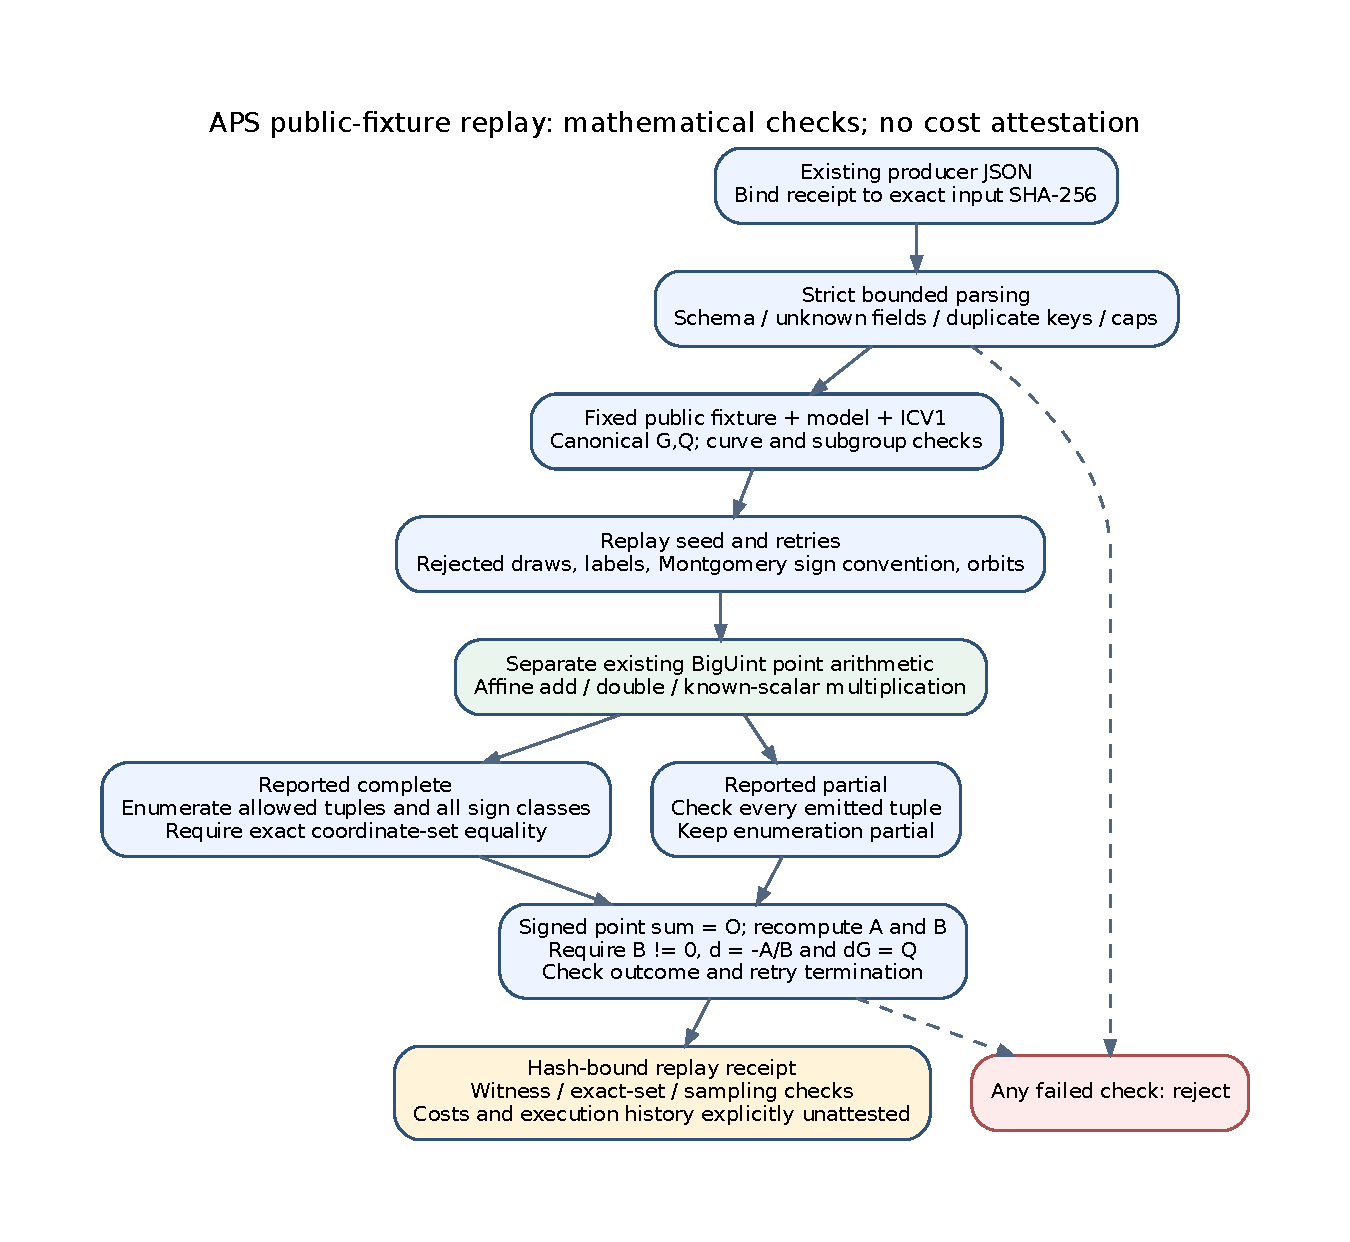
\includegraphics[width=0.94\linewidth,height=0.69\textheight,keepaspectratio]{replay.pdf}
\end{center}

\textbf{Scope of independence.} EC arithmetic and relation checking use a
separate implementation. Serialization, rand 0.8 StdRng and the ICV1 metadata
convention are shared dependencies. The byte hash binds the receipt to the
input, not to a physical execution or a formal proof. The existing partial
Lean coefficient proofs remain unchanged; no new Lean/Rust correspondence
claim is made.

\textbf{Remaining work.} Full operation accounting, native ecbench/export
integration, metric validation, frozen controlled inputs and matched external
solver/rho comparisons remain open. Aborts before a v1 transcript is emitted
are not covered by this replay format. Prior rejected source-checkpoint and
shared-file uploads remain on hold; no performance or EKS job is launched.
The IC leaderboard, performance charts and canonical curve graphs receive no
new values: this work establishes no measured gain or new curve route.

\textbf{Sources.} \href{https://www.secg.org/sec1-v2.pdf}{SEC 1 v2.0},
sections 2.2.1 and 3.2.2.1, for the group law and point validation;
\path{src/ecc/point.rs} and \path{src/ecc/field.rs}, the reused arithmetic;
\path{src/cryptanalysis/aps_single_relation/replay.rs} and
\path{examples/aps_single_relation_check.rs}, implementation and controls.
The earlier APS source map and four-lead study preserve the manuscript,
chord-law references, negative results and formalization boundary.
\end{document}
